% Re-defined by Z.C.TIAN (https://github.com/doem97)
% This version comply with the Official EEE Dissertation Guidline in [EEE dissertation] (http://www.eee.ntu.edu.sg/programmes/CurrentStudents/Graduate_Coursework/mscProg/disHome/Pages/home.aspx)
% More information about dissertation can be found in [NTU thesis](http://research.ntu.edu.sg/rieo/RI/Pages/Theses--Dissertations.aspx)
% Based on W.M.ZHAO version, original link in overleaf:
% (https://www.overleaf.com/latex/templates/ntu-master-dissertation/ngnhrrwryccv)

\documentclass[12pt]{report}

%% Useful packages
\usepackage[a4paper,top=3cm,bottom=3cm,left=3.5cm,right=3cm,marginparwidth=1.75cm,headheight=22pt]{geometry}
\usepackage{amsmath}
\usepackage{cite}
\usepackage{courier}
\usepackage{minted} % For highlighted source code
\usepackage[titletoc]{appendix}
\usepackage[export]{adjustbox}
\usepackage[nottoc,notlot,notlof]{tocbibind}
\usepackage[labelfont=bf, textfont=bf]{caption}
\usepackage{graphicx}
\usepackage{booktabs}
\usepackage[bottom]{footmisc}
\usepackage{hyperref}
\usepackage{float}
\usepackage{setspace}
\usepackage{subfigure}
\usepackage{setspace}
\usepackage{lipsum}
\usepackage{fancyhdr} % Fancy header
\usepackage{url}
\usepackage{tabularx}
\usepackage[utf8]{inputenc}
\usepackage{mathptmx} %Times Font

%add for myself
\usepackage{fontspec}
\usepackage{times}
\usepackage{courier}
\setmainfont{TeX Gyre Termes}
\usepackage{textcomp}

%==== Header and Footer configure ====
% Define the plain pagestyle used by most chapters
\fancypagestyle{plain}{
\fancyhf{} % Clear header footer
\fancyhead[R]{\bf \small \textsl{\nouppercase{\leftmark}} \vspace{0.1in}}
\fancyfoot[R]{\thepage}
% Set the right side of the footer to be the page number
\renewcommand{\headrulewidth}{2pt}
}

%==== Overall Config ====
\setlength{\parindent}{0in} % Set paragraph indent as 0
% \setlength{\fboxsep}{-0.3in}%
\setlength{\fboxrule}{0.5pt} % Set the bounding box around the image as 0.5pt
\pagestyle{plain}
% \renewcommand{\chaptermark}[1]{\markboth{#1}{}}% Comment this line to use header "Chapter 1. Literature View"; otherwise header is "Literature View"



\begin{document}
\fontdimen2\font=0.5em% inter word space
%==== FRONT PART====

%comment begin 
%\begin{titlepage}
	
	\begin{figure}[h!]
		\centering
		
\includegraphics[width=1\textwidth]{Title/NTU_logo.png}
		\caption*{}
		\label{fig:entropy} 
	\end{figure}
	
	\vspace{1.5in}
	
	\centering
	\Huge{\textbf{On MCM\\Principle Part}}\\[2.5in]
	
	\normalsize{\textbf{ZHU HONGRUI, YANG YANJUN, ZOU ZHILI}}\\[0.5in]
	
	%\normalsize{\textbf{SCHOOL OF ELECTRICAL AND ELECTRONIC ENGINEERING}}\\[0.2in]
	
	\textbf{A REPORT SUBMITTED AS AN ASSIGNMENT OF\\EE6610 INTEGRATED CIRCUIT (IC) PACKAGING 21S2}\\[0.25in]
	
	\large{\textbf{2021}}
\end{titlepage}
\newpage % Coverpage
%\begin{titlepage}
\begin{center}
\vspace*{2in}
\Huge{\textbf{Your Title of the Dissertation\\Also Second Line}}\\[2.5in]

\LARGE{\textbf{\MakeUppercase{YOUR NAME}}}\\[1in]

\normalsize{\textbf{\MakeUppercase{SCHOOL OF ELECTRICAL AND ELECTRONIC ENGINEERING}}}\\[0.5in]
\normalsize{\textbf{\MakeUppercase{A DISSERTATION SUBMITTED IN PARTIAL FULFILMENT OF\\THE REQUIREMENTS FOR THE DEGREE OF\\MASTER OF SCIENCE IN XXX}}}\\[0.75in]

% \textbf{A DISSERTATION SUBMITTED IN PARTIAL FULFILMENT OF\\
% THE REQUIREMENTS FOR THE DEGREE OF\\
% MASTER OF SCIENCE IN DIGITAL MEDIA TECHNOLOGY}\\[0.25in]

\large{\textbf{2021}}
\end{center}
\end{titlepage}
\newpage % Titlepage
%\begin{titlepage}

\begin{center}
\Large{\bf{Statement of Originality}}
\end{center}

\vspace{0.2in}

\begin{spacing}{2}

I hereby certify that the work embodied in this thesis is the result of original research and has not been submitted for a higher degree to any other University or Institution.

\end{spacing}

\vspace{2.5cm}

\begin{center}
	\makebox[4cm]{\dotfill}  \hfill \makebox[4cm]{\dotfill}\\
	\makebox[4cm]{Date}      \hfill \makebox[4cm]{Your Name}
\end{center}
\end{titlepage}
\newpage % Titlepage
%\begin{titlepage}

\begin{center}
\Large{\bf{Supervisor Declaration Statement}}
\end{center}

\vspace{0.2in}

\begin{spacing}{2}
I have reviewed the content and presentation style of this thesis and declare it is free of plagiarism and of sufficient grammatical clarity to be examined. To the best of my knowledge, the research and writing are those of the candidate except as acknowledged in the Author Attribution Statement. I confirm that the investigations were conducted in accord with the ethics policies and integrity standards of Nanyang Technological University and that the research data are presented honestly and without prejudice
\end{spacing}

\vspace{2.5cm}

\begin{center}
	\makebox[4cm]{\dotfill}  \hfill \makebox[4cm]{\dotfill}\\
	\makebox[4cm]{Date}      \hfill \makebox[4cm]{Supervisor's Name}
\end{center}
\end{titlepage}
\newpage % Titlepage
%\begin{titlepage}

\begin{center}
\Large{\bf{Authorship Attribution Statement}}
\end{center}

\vspace{0.2in}

\begin{spacing}{2}

This thesis does not contain any materials from papers published in peer-reviewed journals or from papers accepted at conferences in which I am listed as an author.

\end{spacing}

\vspace{2.5cm}

\begin{center}
	\makebox[4cm]{\dotfill}  \hfill \makebox[4cm]{\dotfill}\\
	\makebox[4cm]{Date}      \hfill \makebox[4cm]{Your Name}
\end{center}
\end{titlepage}
\newpage % Titlepage
%comment end

%\begingroup
%\let\cleardoublepage\clearpage

\pagenumbering{roman}

\renewcommand*\contentsname{\centering Table of Contents}
\tableofcontents
\newpage

%comment begin 
%%=== FRONT PART ===
%=== ABSTRCT ===
\newpage

\chapter*{\centering Abstract}
\markboth{Abstract}{}
% \vspace{-0.3in}

\begin{spacing}{1.5}
\setlength{\parskip}{0.3in}

\addcontentsline{toc}{chapter}{Abstract}

Put your abstracts here. The Abstract should be a short and concise passage on the important work and contributions of the project: the motivation and the problem pursued, the method you employed and the results obtained, highlighting the significant achievements. It should not contain peripheral things like summary of literature review, and it is not good enough to say that a certain issue has been studied without stating the results of the study. Generally, one page is about the right length for the Abstract.

\par
\textbf{Keywords:} Dissertation, keywords.
\end{spacing}
\newpage
%=== END OF ABSTRACT ===

%%=== FRONT PART ===
%=== ACKNOWLEDGEMENT ===

%\begin{center}
\chapter*{\centering Acknowledgements}
\markboth{Acknowledgements}{}
\begin{spacing}{1.5}
\setlength{\parskip}{0.3in}
%\end{center}
\addcontentsline{toc}{chapter}{Acknowledgement}

Acknowledgements is to express thanks and appreciation for those who helped in this project.

\end{spacing}
\newpage
%=== END OF ACKNOWLEDGEMENT  ===

%comment end 
%=== FRONT PART ===
%=== ACRONYMS ===
%\begin{center}
\chapter*{\centering Acronyms (template)}
\markboth{Acronyms}{}
\begin{spacing}{1.5}
\setlength{\parskip}{0.3in}
%\end{center}
\addcontentsline{toc}{chapter}{Acronyms}

\begin{table}[ht]
\centering
% \resizebox{0.8\textwidth}{!}{% Uncomment to set fixed width
\begin{tabular}{ll}
\textbf{NN} & Neural Network \\
\textbf{ML} & Machine Learning \\
\textbf{DL} & Deep Learning \\
\textbf{FCN} & Fully Convolutional Network \\
\textbf{CNN} & Convolutional Neural Network \\
\textbf{RCNN} & Region Based Convolutional Neural Network \\
\textbf{DCNN} & Deep Convolutional Neural Network
\end{tabular}%
% }
\end{table}

\end{spacing}
\newpage
%=== END OF ACRONYMS ===

%=== FRONT PART ===
%=== SYMBOLS ===
%\begin{center}
\chapter*{\centering Symbols}
\markboth{Symbols}{}
\begin{spacing}{1.5}
\setlength{\parskip}{0.3in}
%\end{center}
\addcontentsline{toc}{chapter}{Symbols}

\begin{table}[ht]
\centering
% \resizebox{0.8\textwidth}{!}{% Uncomment to set fixed width
\begin{tabular}{ll}
\textbf{$\Pi$} & An Pi Symbol\\
\textbf{$\beta$} & An Beta Symbol\\
\textbf{$\sigma$} & An Sigma Symbol\\
\textbf{$\alpha$} & Another Alpha Symbol\\
\end{tabular}%
% }
\end{table}

\end{spacing}
\newpage
%=== END OF ACKNOWLEDGEMENT  ===



%comment begin 
%\renewcommand{\listfigurename}{\centering List of Figures}
%\listoffigures
%\addcontentsline{toc}{chapter}{Lists of Figures}
%\newpage
%
%\renewcommand{\listtablename}{\centering List of Tables}
%\listoftables 
%\addcontentsline{toc}{chapter}{Lists of Tables}
%\newpage
%comment end 

%\endgroup

%==== MAIN PART ====

\pagenumbering{arabic}
%=== CHAPTER ONE (1) ===
%=== INTRODUCTION ===

\chapter{History and criteria}
\begin{spacing}{1.5}
\setlength{\parskip}{0.3in}

Multi-Chip-Modules have been around since the early 1970s and 1980s mainly used in IBM mainframes first as memory and then for thermal conduction, but have been much wider use in the 1990s. This is an important engineering enhancement that allows the miniaturization of electronic components while improving performance. 

\section{MCM used in early stage}

Multi-Chip-Modules was first introduced into bubble memory in the 1970s. Bubble memory is a type of non-volatile computer memory that uses a thin film of a magnetic material to hold small magnetized areas, known as bubbles or domains, each storing one bit of data. The magnetic material is arranged into parallel tracks and the bubbles can form a serial of ‘1’ and ‘0’ under the control of external field. To increase the density of bubble memories, memory chips were assembled in multilayer stack. This is the original form of MCM. However, the lack of stability and its non-moving characteristics made it obsolete and finally replaced by other memories in 1990s. The idea of MCM was reserved and was used in later technologies.

MCM was also used in mainframe computer packaging. In the 1980s, MCM substrate was first used in this area in the form of Thermal Conduction Module(TCM) which was introduced by IBM. The usage of MCM was not only aim to integrate more chips together, but also to optimize the power distribution, interconnection and cooling. \autoref{fig:TCMwatercool} shows an exploded view of a water-cooled TCM substrate.\cite{Mainframe_Packaging_TCM} From the 1980s to 1990s, IBM TCM technology updated two generations, Alumina-Mo Ceramic MCM and Glass-ceramic copper Ceramic MCM. The third generation will move towards more layers, more I/Os and thinner.

\begin{figure}[ht]
	\centering
	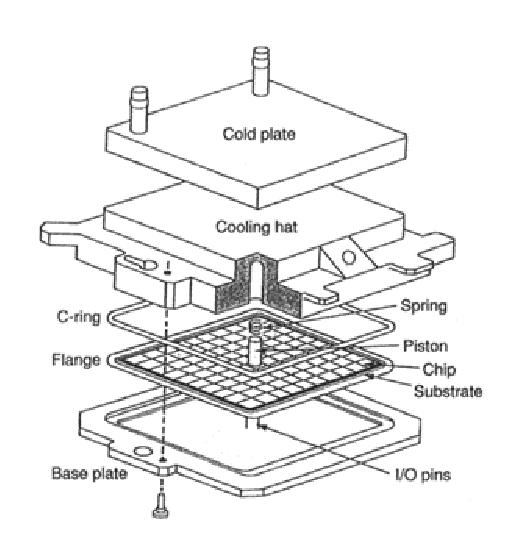
\includegraphics[width=4in, fbox]{Chapter1/TCM_substrate.eps}
	\caption{Exploded view of a water-cooled TCM substrate.(Ref. \cite{Mainframe_Packaging_TCM}, Fig. 13.3 )}
	\label{fig:TCMwatercool} 
\end{figure}

The multilayer ceramic approach derived from TCM was then used to enhance the strength, increase electrical transition speed and reduce the cost of the module. Superconducting multilayer multichip module arises at the right moment. In the 1990s, StratEdge Corporation cooperated with TRW Superconductive Electronic Research Group to provide high performance multichip modules using high-temperature superconductors.\cite{High_temperature_superconducting} Superconducting MCMs were verified to have the performance of high speed, low capacitive impedance, low input-output mismatch and less cable losses. These characteristics were important for developing MCMs in the next several decades.

\section{Recent situation}

Intel also tried several times on the technology of MCM in order to realize the dual-core processor. In 2005, Pentium D, a type of processor in 8xx and 9xx formats, was first introduced during the Intel Developer Forum (IDF). There were two processor die named “Cedar Mill” being integrated inside one Pentium D. At the same time, AMD also released its first dual-core processor, Opteron, in April, 2005. However, AMD made it dual-core in the level of raw wafer and made no use of MCM. Although multi-core can be realized in the absence of MCM packaging technology, MCM packaging can better promote product renewal. For example, the first quad-core processor was manufactured using bare die integration and MCM integration simultaneously.

Nowadays, MCM packaging technology is gradually well developed and has a good application in various fields. In addition to the core processor, GPU, DRAM, etc., are also using MCM technology. We can summarize the development history of so many years and draw the conclusion from the following aspects:

\begin{enumerate}
	\item Higher inter-chip transmission efficiency. Intel Pentium D and IBM both used MCM technology for efficiency. Efficiency is first, then integration.
	\item Higher integration and the race of multi-core. In order to speed up the updating, Intel not only used the multi-core integration of raw wafer, the technique of MCM packaging was also developed and used.
	\item Flexible and accelerated development. To some extent, MCM packaging can make up for the lack of wafer processing development. Multi-core processor, for example, can be fabricated on wafer level or integrated during packaging, which allows companies to launch products in a more flexible way.
\end{enumerate}



\section{Dielectrics}

Polymeric dielectrics have been widely accepted as materials of choice for inter-layer dielectrics in MCMs \cite{Principles_of_Electronic_Packaging}. The higher the dielectric constant of polymeric dielectric is, the higher packaging densities will be achieved. On the contrary, lower or non-uniform dielectric constant will exhibit the characteristic of weaken signal level and cause energy loss. In this case, non-uniform means the dielectric constant varies at different frequency electromagnetic sine wave. If the signal is made up of wave forms of multiple frequencies, the dielectric constant under each component frequencies should take into consideration. In addition, crosstalk also need to be examined. The dielectric constant between two signal lines plays an important role in this case. If the dielectric constant of the material is low enough, the signal lines can be placed very closely.

In the multilevel thin film structures, there are at least two signal layers which can influence each other during the operation. A dielectric layer is a must to serve as an inter-layer to minimize the crosstalk. More specifically, the expected dielectric constant of the dielectric layer should range from 2 to 3.5 and does not vary significantly with frequency (on the order of 0.1) for many of the polymeric dielectrics used in electronic packaging.


\section{Thermal Design}

Temperature is one of the most important player in MCMs as well as other chips. However, it is hard to define the thermal property using only few parameters. All that is wanted is a more suitable working environment for chips and improve the reliability of MCMs. 

There are still some important parameters or concepts need to be mentioned. First is thermal paths. It is obvious that MCMs temperature can be effected by internal and external factors. The internal thermal path is directly formed by the structure itself and heat can transfer from the inside to the outside though it. Also, external temperature and heat dissipation are important but not decide by MCMs. Usually, thermal design follows the experiments and simulations. The experiments gives a briefly direction for the thermal design and computer simulation provide a more specific module to illustrate the thermal path better. Second, heat transfer mechanisms. There are three types of heat transfer: conduction, convection and radiation. The heat conduction is defined by the Fourier cooling law which provide a connection between energy, temperature and parameters of chips. Convection and radiation heat transfer is decide by the external factors such as heat dissipation materials and air or fluid velocity. The last is thermal coupling. In most cases, chips are assembled on the motherboard or PCB board and then installed inside certain cages or on shelves. If there are multiple boards connected to only one backplane, the thermal conduction can be huge and the heat transmission rate is too limited from the plane to the ambient to sustain the significant heat generation. Frames or enclosures are designed to deal with the thermal coupling. 

There are several thermal control methods could be used for MCMs. Material property improvement is the most effective way to deal with thermal problems. If the thermal resistance can be reduced by changing materials, the heat will spread more quickly and leave MCMs operating in a lower temperature. However, this approach is constrained by a number of factors. So, people come up with other ideas such as backside cooling. A metal mount is usually attached at the backside of MCMs to transfer heat to the ambient more efficiently. Then, many methods, natural convection, forced convection, liquid immersion, etc. can be applied to cool the chip down.

\section{Electrical Design}

There are a set of electrical parameters to be considered during the fabrication of MCMs, such as delay, noise, reflection, crosstalk, line losses, loading effect and so on. The final objective of the electrical design of MCM is to produce a layout which is a description of the artwork used to make the masks to be applied in MCM production.\cite{Doane1993MultichipMT}

With the aid of computers, we can follow the process shown in \autoref{fig:layoutflowchart} to prepare the layout of MCMs. Start with timing design and then fulfill the requirements of net delay. After MCM placement and routing there is a process of back annotate. Finally, the simulation of timing verification and signal integrity will give out the result of the layout assessment.
\newpage
\begin{figure}[ht]
	\centering
	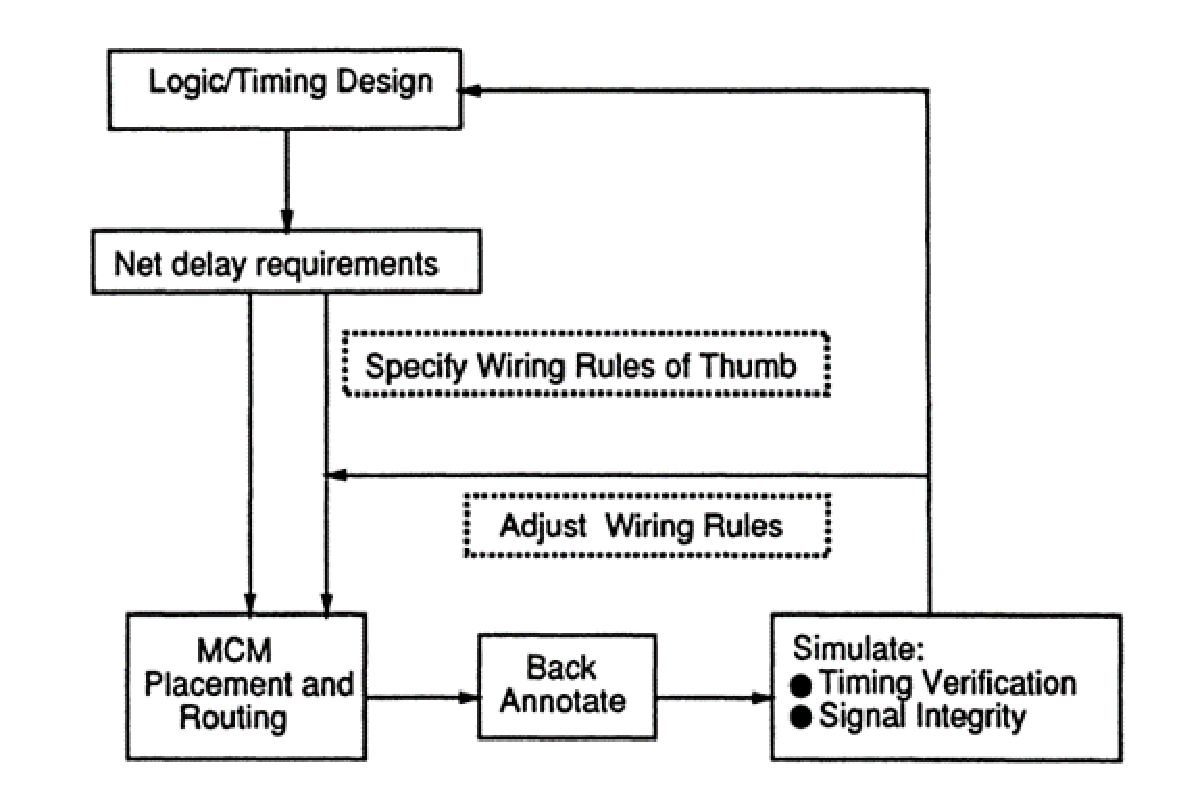
\includegraphics[width=4in, fbox]{Chapter1/layout_flow.eps}
	\caption{The steps in producing an MCM layout.(Ref. \cite{Doane1993MultichipMT}, Fig. 11.22 )}
	\label{fig:layoutflowchart} 
\end{figure}

About the noise control, noise on data signal lines can be fixed to some extent but excess noise on clock lines should be eliminated. The delay on the data path is contributed by the impedance and the length of the line as well as the properties of dielectric layers. A short path and low line resistance would be preferred to minimize the internal delay. Reflection and crosstalk also need to be treated well which involves carefully design of the layout and interconnections. Delay and noise have great influence on chip performance and can be reduced by using MCM technology. So, MCM packaging is a comprehensive technology which needs to take into account many electrical properties. 



\end{spacing}
%=== END OF CHAPTER ONE ===
\newpage



%=== CHAPTER TWO (2) ===
%=== Literature Review ===

\chapter{Methodology}
\begin{spacing}{1.5}
\setlength{\parskip}{0.3in}

After an introduction on the development history and a brief on design criteria, this chapter focuses on specific components. For the rest of this chapter, the analysis of MCM will go deeper into explanations for key MCM design methodologies, thus giving a detailed view on MCM design. 

\section{Package Style}

assembly techniques (surface mount, chip and wire) 9.11 p.223 

Assembly, the macro arrangement of MCM structure, determines existances of specific conponents. After several decades of MCM development, various methods of assembly have been implemented, with costs and performances ranging from low to high. 

Traditionally, industrial attention has been paid on the surface-mount assembly method, which provides a considerable performance with the lowest cost. This technique solders pre-packages components onto intended substrates to form the overall module. Many package styles can be categorized as this method: SIP, DIP, etc. 

To integrate circuits and components onto the substrate via expoxy attachment and wire bonding provides another method with higher density as well as a very low interconnect electronic circuit parasitics. This is called the chip-and-wire assembly, and it can be implemented through various package styles, e.g., epoxy seal, metal package. 

The above techniques can also be applied at the same time to form a hybrid package. \cite{licari1998hybrid}

Three main methods for IC die attachment are provided in current industries: wirebond, flip chip and TAB. \cite{bogatin1997roadmaps} 

%\begin{enumerate}
%    \item 
%\end{enumerate}

Regarding to the thermal design mentioned in the previous part, it's important to take the heat spreader into consideration. 

e.g.

• Epoxied directly to the BeCu heat spreader through a cutout in the board
• Epoxied to the head spreader, through a cutout, via a thermally conductive submount, to electrically isolate the die from the heat spreader

The package style of an MCM should be designed according to its practical usage. Major considerations towards the design scheme should include and should not be limited to: on the frontend, the general function, purpose, interconnects, testability, available assembly techniques, active elements configurations; on the backend, placement, routing, via minimization, tree searching, layer estimation, potential failure risks, reliability. 

Hence, during the design flow, careful attention must be paid on the arrangements of these technologies, so that appropriate ones can be applied on appropriate places. \cite{chen2006vlsi} 

\section{Wiring}

Wiring in MCM supports one of its critical funcitons: to provide both signal interconnects for the chips within the package and an interface between the module itself and the outer environment. In current industrial applications, there are three mainstream metals for MCM wiring fabrication: Al (aluminum), Cu (copper) and Au (gold). 

\begin{enumerate}
    \item Al is well known for its low fabrication cost and a proper oxidization resistivity. It's easy to sputter and evaporate Al onto the intended surface, but the difficulty in electropolation limits its flexibility. 
    \item Cu has a significantly larger conductivity and a better electromigration resistivity compared with Al, and it's also very flexible in deposition methods. However, oxidization on the surface of copper makes it hard to adhere to other materials, especially dielectrics and other wires. 
    \item Au has the highest conductivity among these materials, making it very suitable for thin-film fabrication. What's more, it has a faily good deposition method flexibility, though its adhesion is poor so that a Ti or Ti/W layer is always needed. Another critical shortcoming is its high cost. 
\end{enumerate} 

Directly related to the wiring fabrication, the conductor materials should be determined in accordance with the design, electrical requirements and process requirements. Among numerous properties of a given material, conductivity and reliability are the most important towards fulfilling the specification. \cite{chen2006vlsi}

\textit{There are also other various types of wiring materials... }

\textit{In the previous chapter, a key considerations for wiring design has been introduced: the wiring density.} In the design flow of an MCM, the need to determine its size usually leads to a \textit{wireability analysis}. 

A wireability analysis includes considerations about three parameters of this design: \textit{wiring demand} (D), \textit{wiring capacity} (C), \textit{average wire length} and \textit{connectivity}. 

The wiring demand refers to the \underline{required} amount of wiring for a given circuit's interconnection, while the wiring capacity indicates the \underline{maximum available} amount. The relationship between them can be expressed as follows: 

\begin{equation}
    \label{eq.demand} 
    D=\epsilon C
\end{equation}

where $\epsilon$ stands for the wiring efficiency with a circuit specified typical value between 30\% to 70\%. Neglecting via and through holes, the total wiring capacity $C_T$ can be described through the following equation, for a given MCM: 

\begin{equation}
    \label{eq.capacity}
    C_T=\frac{P_P\times N_T}{P_S}
\end{equation}

where $P_S$ is the mininum signal line pitch; $P_P$ is the pitch size; $N_T$ is the number of wiring layers. 

The calculation of wiring demand, on the other hand, the average length per interconnection $\overline{L}$, or the Manhattan length, should be estimated beforehand. A classical estimation method by Rickert is 

\begin{equation}
    \label{eq.rickert}
    \overline{L}=0.77P_PN_C^{0.245}
\end{equation}

where $N_C$ is the number of chips to be interconnected. \cite{rickert1989design} 

The number of I/O pins is another crucial parameter in the design stage of an MCM. The well-known Rent's Rule gives a very useful estimation on this 

\begin{equation}
    \label{eq.rent}
    N_{IO}=ag^b
\end{equation}

In the above equation, if a specific chip is given, $N_{IO}$ is its anticipated number of I/Os; $g$ is its number of gates; $a$ and $b$ are the average connection number per I/O, or the Rent's coefficient, and the Rent's exponent respectively. \cite{landman1971pin} $a$ and $b$ are determined emperically and several typical values are given below. \cite{tummala2001fundamentals}

\begin{table}[ht]
    \centering 
    \caption{Rent's coefficients and exponents for specific devices/systems} 
    \label{tb.rent} 
    \begin{tabular}[t]{lcc}
        \toprule 
        Type & Rent's coefficient, $a$ & Rent's exponent, $b$ \\ 
        \midrule 
        DRAM & 6.20 & 0.085 \\
        SRAM & 6.00 & 0.120 \\ 
        Microprocessors & 0.82 & 0.450 \\ 
        Random Logi & 1.90 & 0.500 \\
        Computer Systems & 2.50 & 0.600 \\ 
        \bottomrule
    \end{tabular}
\end{table}

\textit{Also, \underline{emphasize} their importance}

chip and wire assembly

\section{Substrate}

The whole chapter 9 \cite{chen2006vlsi}

For any packaging design, the substrate influences almost every part of its overall performance. 

C: thick-film, HTCC, LTCC. D: inorganic dielectrics on Si, organic dielectric on Si. L: laminated board

substrate technologies (how to carry dies) 9.10 p.220 \cite{chen2006vlsi} 

%=== END OF CHAPTER TWO ===
\end{spacing}
\newpage


%comment begin 
%%=== CHAPTER THREE (3) ===
%=== (Actual work done and contribution, including literature survey) ===

\chapter{Approach}
\begin{spacing}{1.5}
\setlength{\parskip}{0.3in}
%  (Actual work done and contribution, including literature survey)


\section{One}

The next few chapters should describe the work you have done in tackling the problem. There might be a chapter on the fundamental theories relevant to the solution you are pursuing, or the supporting technologies you need in implementing the solution. Then there should be a chapter on the solution itself, followed by a chapter on the results and analysis of the results

\section{Two}


\section{Three}


%=== END OF CHAPTER THREE ===
\end{spacing}
\newpage

%%=== CHAPTER FOUR (4) ===
%=== Test and Experiments ===

\chapter{Test and Experiments}
\begin{spacing}{1.5}
\setlength{\parskip}{0.3in}

\section{One}


\section{Two}

\section{Three}


%=== END OF CHAPTER FOUR ===
\end{spacing}
\newpage

%%=== CHAPTER FIVE (5) ===
%=== Discussion ===

\chapter{Discussion}
\begin{spacing}{1.5}
\setlength{\parskip}{0.3in}

\section{One}

Generally, there should be no more than six or seven chapters in your dissertation. If you have more than that, you should take a close look at its orgainsation and see if certain chapters can be merged.

\section{Two}

\section{Three}


%=== END OF CHAPTER FIVE ===
\end{spacing}
\newpage

%%=== CHAPTER SIX (6) ===
%=== Conclusion and Recommendations ===

\chapter{Conclusion and Recommendations}
\begin{spacing}{1.5}
\setlength{\parskip}{0.3in}

\section{One}

The last chapter is always the Conclusion. This generally should have three parts. The first is a concise summary of the work you have done. In a way, this is similar to the abstract. Then there is the conclusion, in which you highlight the significance of the results, and perhaps the consequences of the results, critically where necessary. The last thing is usually recommendations and/or future work, in which you identify the inadequacies of what you have done, and suggest how the gaps may be plugged.

\section{Two}

Documents that are prepared with the help of other sources should have a list of sources cited. A list of References contains only sources the writer quotes directly, takes original ideas from, and refers to in the dissertation should be included. In reports where the subject is primarily scientific, the list of references is the most widely accepted way to cite specific sources.

\section{Three}

\section{Four}

\subsection{Six}


%=== END OF CHAPTER SIX ===
\end{spacing}
\newpage

%comment begin 

%==== ENDING PART ===

\renewcommand\bibname{References}
\bibliographystyle{unsrt}
\begin{spacing}{1.5}
\bibliography{Ref/References}
\end{spacing}
\newpage

%comment begin 
%%=== APPENDIX ===

\begin{appendices}
\label{cha:appendices}

\chapter{Introduction of Appendix}
\markboth{Appendix A}{} % For appendix first (affects header)
\begin{spacing}{1.5}

The Appendix contains related data not necessary to the immediate understanding of the discussion in the report. This may contain materials such as: tables, graphs, illustrations, description of equipment, samples of forms, data sheets, questionnaires, equations, and any material that must be included for record purposes.
Each entry (sample forms, detailed data for references, tables, pictures, questionnaires, charts, maps, graphic representations) in the appendix requires an identifying title. Every entry in the appendix must be referred to in the body of the report. Each appendix must be lettered, beginning with Appendix A. The list of appendices should be appearing in the table of contents following the list of references entry.

\end{spacing}

\chapter{Sample Code}
\markboth{Appendix B}{} % For appendix second, etc.. 

below shows how to insert highlighted source code from the source file.

\inputminted[
tabsize=4, % change this to set the spacing of tab
breaklines, % automatically wrap the code
fontsize=\scriptsize % Can be \footnotesize, \small, \normalsize etc
]{python}{Appendix/sample.py}

\end{appendices}
%comment end 
%==== END OF ALL ===
\end{document}
